\newpage
\subsection{Traditional Project Management}
% Explain waterfall model (maybe a little sarcastic painting the perfect world) and then oops yeah
% that's why it is not really working for web projects. Cause working in Silos is bad.
% First quickly explain waterfall model.
% Then say advantages and disadvantages.
% Then say why it is not working for web projects.
%  - After project finish there is a product, but in between there is almost never a working product.
%  - Silos are bad, long handoffs, no way to change design after development started.
%  - No way to react to user feedback.
%  - No way to react to changing requirements.
The most traditional way of managing software projects is the Waterfall model. It breaks down the
project into several phases, where each phase is completed before the next one starts. That means
it is a very linear approach, the project flows from one phase to the next, with handoffs in
between. \vglcite{theinstituteofprojectmanagementWaterfallMethodology2022}

\begin{figure}[H]
      \centering
      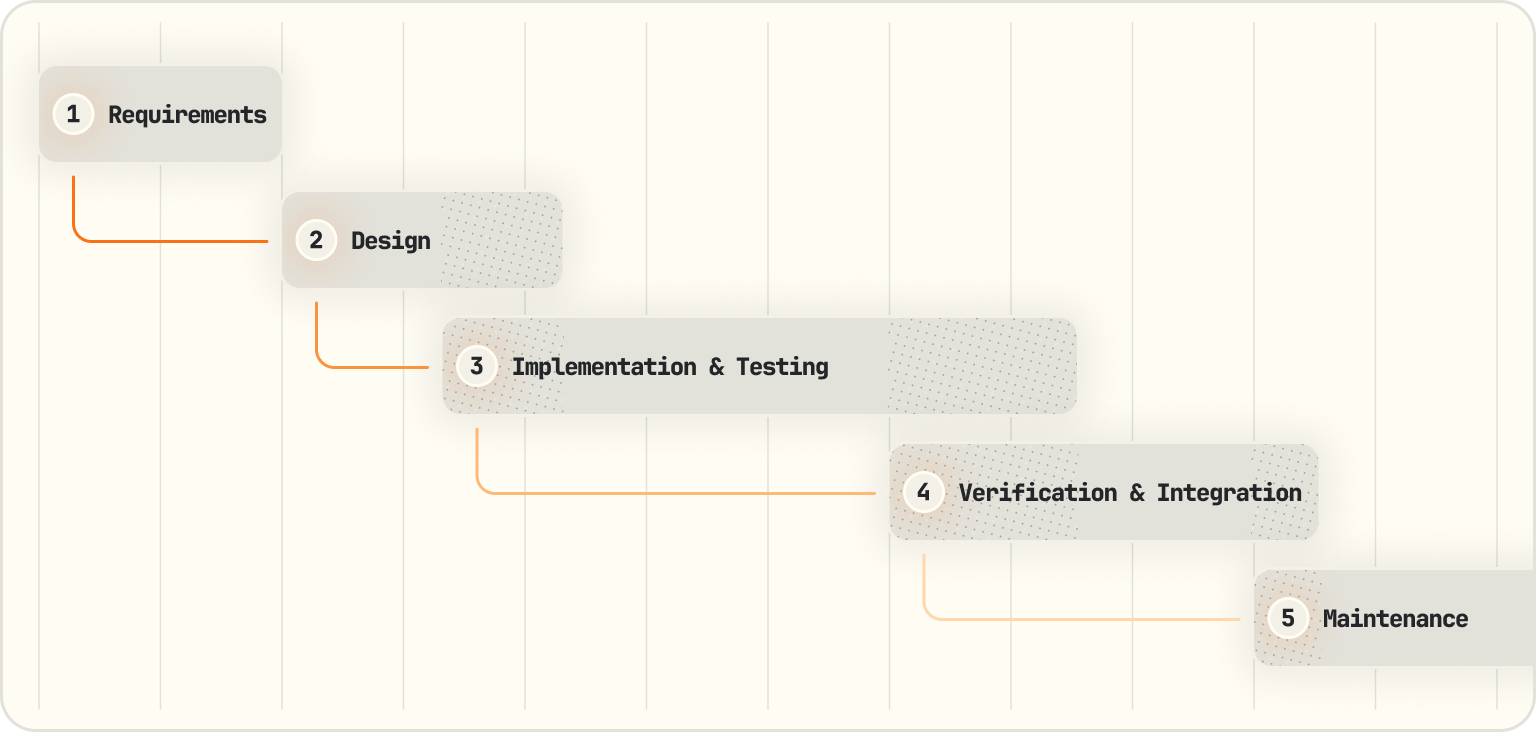
\includegraphics[width=250pt]{Chapter 3/Traditional Project Management.png}
      \caption{Flow of traditional project management (Source: own illustration based on Institue Project Management https://projectmanagement.ie/blog/waterfall-methodology/)}
\end{figure}
For a typical software or web project, the phases are usually something like this: % NOTE DONE: Maybe add a graphic
\begin{enumerate}
      \item \textbf{Requirements}\\
            Conduct research and gather requirements for the project. Collect as much information 
            as possible to then create a detailed project
            plan.\vglcite{theinstituteofprojectmanagementWaterfallMethodology2022} 
      \item \textbf{Design}\\
            Create the design based on the requirements that show how the final product will look
            and how this will be achieved. This includes UI, but also architecture design.
            \vglcite{theinstituteofprojectmanagementWaterfallMethodology2022} 
      \item \textbf{Implementation \& Testing}\\
            Develop the product based on the design and test it to ensure it meets the
            requirements. \vglcite{theinstituteofprojectmanagementWaterfallMethodology2022} 
      \item \textbf{Verification \& Integration}\\
            The product is validated to check if all requirements are met. If everything works,
            the product is launched.
            \vglcite{theinstituteofprojectmanagementWaterfallMethodology2022} 
      \item \textbf{Maintenance}\\
            After launch the product is maintained and updated as needed.
            \vglcite{theinstituteofprojectmanagementWaterfallMethodology2022} 
\end{enumerate}

When looking at the sequence of these phases, it may seem like it is a perfect solution for every kind
of project. However, while this model works especially for projects that have a defined and fixed
scope, many software or web projects do not exactly work that way as the design process alone is by
nature not a one-time thing. Also, teams of different disciplines work separately from each other,
forming rigid silos if documentation is not a top priority.
\vglcite{theinstituteofprojectmanagementWaterfallMethodology2022} 

\subsubsection{Common Problems and Effects of Bad Collaboration}
Despite its structured approach, this model presents significant challenges for fast-paced software
and web development projects in practice. The following are key issues that arise from these
limitations.

\textbf{Long Handoff Meeting} \\
When the design is finished and handed off to the development team, a long meeting is necessary. The
developers need to understand the design from the ground up, which can lead to misunderstandings,
misinterpretations and a lot of back and forth.

\textbf{No end-user prioritization} \\
The focus on meeting requirements first specified, can lead to a product that doesn't comply with
the needs of the user. As there is almost no way to go back and change the design, the products
success is only really revealed after launch which is very risky.

\textbf{No Room for UX Focus} \\
Adding to the previous point, without much end-user feedback usability testing and other UX methods
are cut short making it hard to emphasize UX. Even if usability testing is integrated, it is
extremely costly to go back and change the initial design in later phases such as
implementation.

\textbf{Risk of nothing to show for} \\
\begin{figure}[H]
      \centering
      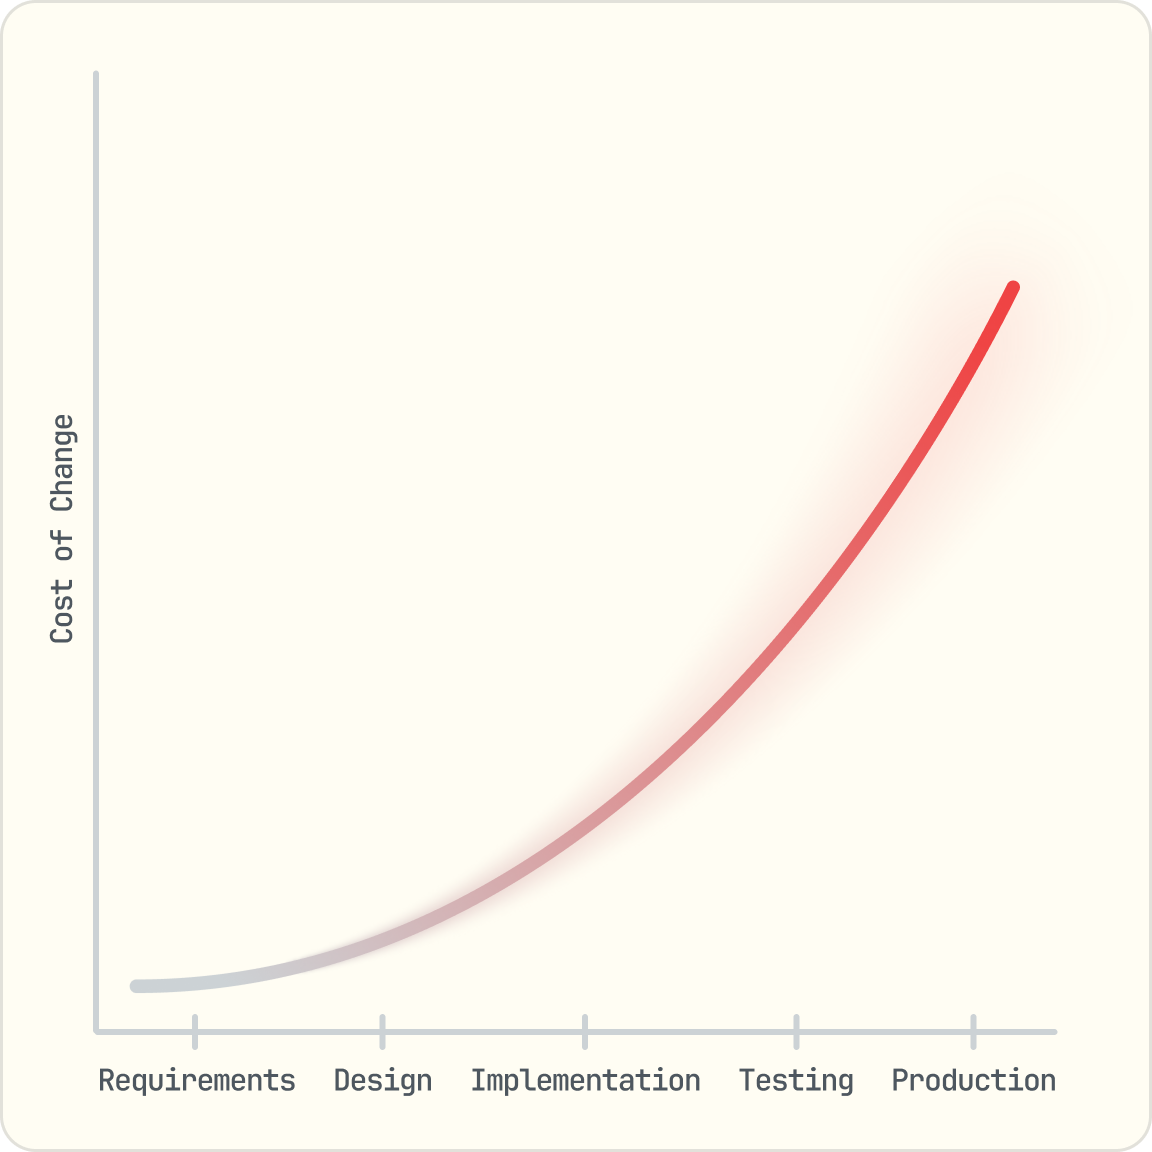
\includegraphics[width=200pt]{Chapter 3/Cost of Change.png}
      \caption{Cost of change over the course of a project (Source: own illustration based on Project Management.com https://www.projectmanagement.com/articles/308195)}
\end{figure}
Another result of the linear, separate team approach is that there is not a working version of the
product for quite some time. So, when the project is cancelled prematurely, there could be nothing
to show for. \vglcite{mikegriffithsIntroductionCostChange2015}
% NOTE DONE: mach so ne grafik rein:
% https://www.google.com/search?sca_esv=61eddb219bf0e5e6&sxsrf=AHTn8zo4RD4tpO9VjZHRDRIlptCIvp0pGQ:1741695083635&q=project+change+cost+over+project+timeline+graph%C3%A4&udm=2&fbs=ABzOT_CWdhQLP1FcmU5B0fn3xuWpA-dk4wpBWOGsoR7DG5zJBkzPWUS0OtApxR2914vrjk4ZqZZ4I2IkJifuoUeV0iQtITiOPPo9tDzmt9ZPGYJiIba3ipclDVbOjJlvTbgEP2s-bkOIhr5ELgbQI8I7zKhriYCgRXaYljMf-YpaNgLRzy2fJ38VbFwBTF_D5ZCA5_SutZQD&sa=X&ved=2ahUKEwiplpHm_4GMAxW6S_EDHckeGToQtKgLegQIFxAB&biw=1680&bih=913&dpr=2#vhid=jRm_exLG44TCIM&vssid=mosaic 
